\chapter{PAKET DATA SPOPD}

Paket data SPOPD dibangun oleh komponen-komponen, dan setiap komponen memiliki struktur seperti pada tabel \ref{tab:paketdata}. Beberapa komponen harus selalu terdapat pada paket data, ada juga yang tidak.

\begin{table}[h!]
  \centering
  \begin{tabular}{| l | l | c |}
    \hline
	\rowcolor{lightgray} Komponen & Panjang & Status \\
    \hline
    Kode Pengenal Paket Data & 4 bytes & required \\
    \hline
    Primary Bit Map & 16 bytes & required \\
    \hline
    Data Element & Variable length & Optional \\
    \hline
  \end{tabular}
  \caption{Tabel Paket Data SPOPD}
  \label{tab:paketdata}
\end{table}

Data element yang disertakan dalam sebuah paket data \textit{incoming} dan \textit{outgoing} dapat dikonfigurasikan secara sendiri-sendiri. SPOPD memiliki sekumpulan konfigurasi paket data yang akan digunakan untuk pengolahan transaksi.

\begin{enumerate}[A.] 
  \item \textbf{\textit{Komponen Paket Data}}
  
  Komponen dan Struktur Paket Data SPOPD dapat dilihat seperti pada gambar \ref{fig:komponenpaketdata}
  
  \begin{figure}[H]
    \centering
    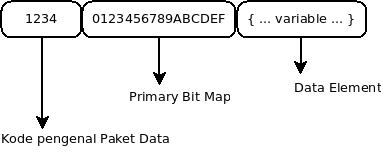
\includegraphics[width=1\textwidth]{./resources/dia-komponen-paket-data}
    \caption{Diagram Paket Data SPOPD}
    \label{fig:komponenpaketdata}    
  \end{figure}
  
  \item \textbf{\textit{Kode Pengenal Jenis Paket Data}}

  Kode pengenal jenis paket data terdiri atas 4 digit karakter yang memberikan gambaran mengenai fungsi paket data yang dikirimkan. Penjelasan rinci mengenai kode pengenal paket data yang digunakan dalam SPOPD dapat dilihat pada pembahasan selanjutnya dalam dokumen ini.
  
  \item \textbf{\textit{Primary Bit Map}} 
  
  \textit{Primary Bit Map} (PBM) adalah merupakan sebuah \textit{field}/atribut yang terdiri atas 16 digit karakter. PBM ini harus selalu terdapat pada setiap paket data yang dikirimkan. PBM merupakan kode yang terdiri atas 64 bit data yang merepresentasikan keberadaan (ditandai dengan '1' atau \textit{bit on}) atau tidaknya (ditandai dengan '0' atau \textit{bit off}) 64 data element pertama dari paket data.
  
  Enam puluh empat bit tersebut dikonversikan ke/dari 16 blok data menggunakan persamaan heksadesimal. Untuk mengkonversikan 64 bit data ke dalam 16 blok data, ke 64 bit data tersebut dikelompokan dalam 16 kelompok yang terdiri atas 4 bit data. Kemudian setiap kelompok bit (4 bit data) dikonversikan menggunakan persamaan heksadesimal.
  
  Tabel persamaan dari bentuk bit / biner ke bentuk heksadesimal dapat dilihat pada tabel \ref{tab:bintohex}
  
\begin{table}[H]
  \centering
  \begin{tabular}{| c | c |}
    \hline
    \rowcolor{lightgray} BIT & HEX \\
    \hline
    0000 & 0 \\
    \hline
    0001 & 1 \\
    \hline
    0010 & 2 \\
    \hline
    0011 & 3 \\
    \hline
    0100 & 4 \\
    \hline
    0101 & 5 \\
    \hline
    0110 & 6 \\
    \hline
    0111 & 7 \\
    \hline
    1000 & 8 \\
    \hline
    1001 & 9 \\
    \hline
    1010 & A \\
    \hline
    1011 & B \\
    \hline
    1100 & C \\
    \hline
    1101 & D \\
    \hline
    1110 & E \\
    \hline
    1111 & F \\
    \hline
  \end{tabular}
  \caption{Tabel Persamaan Biner ke Heksadesimal}
  \label{tab:bintohex}
\end{table}

Di bawah ini adalah contoh bagaimaan 64 bit data dikonversikan ke dalam 16 blok data. Kode bit data dimulai dari kiri sebagai bit pertama yang memberikan keberadaan data element ke-1.

\tiny{
\begin{tabu} to 1\textwidth{ X[c] X[c]X[c]X[c]X[c] X[c]X[c]X[c]X[c] X[c]X[c]X[c]X[c] X[c]X[c]X[c]X[c] X[c]X[c]X[c]X[c] X[c]X[c]X[c]X[c] X[c]X[c]X[c]X[c] X[c]X[c]X[c]X[c]}
\multicolumn{25}{c}{Bagian Pertama} \\
&1&2&3&4&5&6&7&8&9&0& 1&2&3&4&5&6&7&8&9&0& 1&2&3&4&5&6&7&8&9&0& 1&2 \\
Bit Map:&0&0&1&0 &0&0&1&0 &0&0&0&1 &1&0&1&0 &0&1&0&0 &0&0&1&1 &0&0&0&0 &0&0&0&0 \\
PBM: &\multicolumn{4}{c}{2} &\multicolumn{4}{c}{2} &\multicolumn{4}{c}{1} &\multicolumn{4}{c}{A} &\multicolumn{4}{c}{4} &\multicolumn{4}{c}{3} &\multicolumn{4}{c}{0} &\multicolumn{4}{c}{0} \\[1em]
\multicolumn{25}{c}{Bagian Kedua} \\
&1&2&3&4&5&6&7&8&9&0& 1&2&3&4&5&6&7&8&9&0& 1&2&3&4&5&6&7&8&9&0& 1&2 \\
Bit Map:&0&0&0&0 &0&1&0&1 &0&0&1&0 &0&0&1&1 &0&1&1&0 &1&1&1&1 &1&0&1&1 &1&1&0&1 \\
PBM: &\multicolumn{4}{c}{0} &\multicolumn{4}{c}{5} &\multicolumn{4}{c}{2} &\multicolumn{4}{c}{3} &\multicolumn{4}{c}{6} &\multicolumn{4}{c}{F} &\multicolumn{4}{c}{B} &\multicolumn{4}{c}{D}
\end{tabu}
}
  
  Berdasarkan contoh di atas, \textit{Primary Bit Map} memiliki nilai: 221A430005236FBD. PBM di atas memberikan informasi keberadaan data element :

\begin{italicquotes}
{3, 7, 12, 13, 15, 18, 23, 24, 38, 40, 43, 47, 48, 50, 51, 53, 54, 55, 56, 57, 59, 60, 61, 62, 64}
\end{italicquotes}

  ada dua jenis kode bit map yang digunakan dalam standar paket data SPOPD yang dinamakan sebagai \textit{Primary} (PBM) dan \textit{Secondary Bit Map}(SBM). PBM digunakan untuk merepresentasikan keberadaan data elemen 1 s/d 64, sedangkan SBM digunakan untuk merepresentasikan keberadaan data elemen 65 s/d 128. PBM diletakan setelah kode pengenal jenis paket data, mendahului data elemen. Sedangkan SBM adalah merupakan data elemen ke-1 (P-1) yang keberadaannya dapat diketahui melalui PBM.
  
  \item \textbf{\textit{Data Elemen}}
  
  ISO 8583 \textit{message exchange standard} memiliki 128 data elemen. Dalam sistem SPOPD tidak semua data elemen digunakan. Konfigurasi data elemen yang diikutkan pada setiap paket data bervariasi menyesuaikan dengan pemrosesan yang akan dilakukan. Secara rinci data elemen yang digunakan untuk setiap paket data dapat dilihat pada pembahasan selanjutnya dalam dokumen ini.
\end{enumerate}